% Inbuilt themes in beamer
\documentclass[12pt]{beamer}

% --- añadidos mínimos para pdfLaTeX ---
\usepackage[utf8]{inputenc}
\usepackage[T1]{fontenc}
\usepackage{lmodern}
\usepackage[spanish]{babel}
\usepackage{amsmath, amsfonts, amssymb, amsbsy}
\usepackage{mathrsfs} % para formato de letra
\usepackage{ragged2e}
\usepackage{hyperref}
\usepackage{float}
\usepackage{url}
\setbeamertemplate{caption}[numbered]
% --------------------------------------

% --- TEMA Y DATOS ---
\usetheme{Madrid}

\title{Artificial Lemming Algorithm (ALA)} 
\author{Pardo. M, Pérez. J, Saldivia. J, Sandoval. S}
\date{29 de agosto de 2025}

\begin{document}

% Portada (1 diapo)
\begin{frame}
  \titlepage
\end{frame}

% Índice (2 diapo)
\begin{frame}{Contenido}
  \tableofcontents %Esto se pone automático para tener más claro las secciones, hay que poner \section
\end{frame}

% ===== Ejemplo de sección y frame =====
\section{Introducción}

\begin{frame}{Introducción}
  \begin{block}{Artificial Lemming Algorithm}
      \justifying
      \begin{itemize}
          \item Desarrollado por  Yaning Xiao, Hao Cui, Ruba Abu Khurma, Pedro A. Castillo
          \item Es una metaheurística basada en el comportamiento biológico de los Lemmings
          \item Se inspira en cuatro conductas claves: Migración a larga distancia, Excavación de madrigueras, Forrajeo de alimento y Evasión de depredadores
          \item Sus soluciones iniciales se generan aleatoriamente y el algoritmo equilibra exploración y explotación mediante un factor de energía decreciente
          \item Incorpora técnicas como movimiento browniano y vuelo de Lévy para mejorar la diversidad y evitar óptimos locales
          
      \end{itemize}
      
  \end{block}
\end{frame}


\section{Inicialización}
\begin{frame}{Inicialización}
    \justifying
    \begin{itemize}
        \item La población inicial se genera de manera aleatoria dentro de los límites del problema.
        \item Cada individuo representa una posible solución en un espacio de dimensión $d$.
        \item Esta diversidad inicial permite cubrir de forma amplia el espacio de búsqueda.
    \end{itemize}

    \vspace{0.5em}
    \begin{columns}[c]
        % Columna izquierda: matriz (Eq. 3)
        \column{0.5\textwidth}
            \centering
            \includegraphics[width=0.9\linewidth]{Ecuacion3.png}
            \vspace{0.3em}
            {\scriptsize Matriz de soluciones iniciales (Eq. 3)}

        % Columna derecha: ecuación (4)
        \column{0.5\textwidth}
            \begin{equation*}
                z_{i,j} = LB_j + rand \times (UB_j - LB_j)
            \end{equation*}
            \vspace{0.3em}
            \small
            {\scriptsize Con $rand$ entre [0,1] y $LB_j$, $UB_j$ limítes superior e inferior  (Eq. 4)}
    \end{columns}
\end{frame}

\section{Estructura}

\begin{frame}{Estructura general }
  \begin{block}{Exploración, Explotación y Energía}
      \justifying
      \begin{itemize}
          \item El ALA combina 4 comportamientos de los lemmings → 2 de exploración y 2 de explotación
          \item La elección depende del factor de energía $E(t)$
          \item Si $E > 1$ : Exploración
          \item Si $E <= 1$ : Explotación
          \item El factor de energía decrece con las iteraciones, permitiendo una transición natural entre fases
          \begin{equation*}
              E(t) = 4 \times \arctan\!\left( 1 - \frac{t}{T_{\text{max}}} \right) 
       \times \ln\!\left( \frac{1}{rand} \right) \tag{17}
          \end{equation*}
      \end{itemize}
  \end{block}
\end{frame}

\begin{frame}{Exploración }
  \begin{block}{Migración a larga distancia}
      \justifying
      \begin{itemize}
          \item Cuando hay escasez de recursos, los lemmings realizan migraciones largas y aleatorias.
          \item Cada agente combina su posición actual, un individuo aleatorio y un ruido browniano → lo que permite explorar nuevas zonas.
          \item La dirección y la distancia de la migración no son estáticas. 
      \end{itemize} 
  \end{block}
  \small
  \begin{equation*}
\vec{Z}_{i}(t+1) = \vec{Z}_{best}(t) 
+ F \times \overrightarrow{BM} \times 
\Big( \vec{R} \times \big( \vec{Z}_{best}(t) - \vec{Z}_{i}(t) \big) 
+ (1 - \vec{R}) \times \big( \vec{Z}_{i}(t) - \vec{Z}_{a}(t) \big) \Big)  \tag{5}
\end{equation*}
\end{frame}

\begin{frame}{Exploración }
  \begin{block}{Excavar madrigueras}
      \justifying
      \begin{itemize}
          \item Los lemming excavan nuevas madrigueras de forma aleatoria basándose en su ubicación actual y en la posición de individuos aleatorios de la población
          \item Se regula a través de $L$ y $F$ la profundidad y sentido del túnel
      \end{itemize}
  \end{block}
  \begin{equation}
\vec{Z}_i(t+1) = \vec{Z}_i(t) + F \times L \times \left( \vec{Z}_{best}(t) - \vec{Z}_i(t) \right) \tag{9}
\end{equation}

\end{frame}

\begin{frame}{Explotación }
  \begin{block}{Forrajeo de comida}
      \justifying
      \begin{itemize}
          \item Los lemmings se mueven aleatoriamente dentro de su área de forrajeo para encontrar fuentes de comida, utilizando su agudo sentido del olfato y oído.
          \item El área de forrajeo se establece dependiendo de la abundancia de alimentos y la distancia de la solución óptima encontrada previamente.
      \end{itemize}
  \end{block}
  \begin{equation}
\vec{Z}_i(t+1) = \vec{Z}_{best}(t) + F \times \text{spiral} \times \text{rand} \times \vec{Z}_i(t)
\tag{11}
\end{equation}
\end{frame}

\begin{frame}{Explotación }
  \begin{block}{Evadir depredadores}
      \justifying
      \begin{itemize}
          \item Cuando los lemmings se enfrentan a un depredador, utilizan su agilidad para huir hacia la madriguera.
          \item Realizan maniobras engañosas utilizando el vuelo de Lévy para evitar la persecución y escapar hacia un punto seguro.
      \end{itemize}
  \end{block}
  \begin{equation}
\vec{Z}_i(t+1) = \vec{Z}_{best}(t) + F \times G \times \text{Levy(Dim)} \times \left( \vec{Z}_{best}(t) - \vec{Z}_i(t) \right)
\tag{14}
\end{equation}
\end{frame}

\section{Diagramas y Pseudocódigo}
\begin{frame}{Diagrama de flujo }
  \centering
            \includegraphics[width=0.9\linewidth]{DiagramaFlujo.png}
\end{frame}

\begin{frame}{Pseudocódigo }
  \centering
            \includegraphics[width=0.8\linewidth]{Pseudocódigo.png}
\end{frame}

\section{Aplicaciones en la vida real}
\begin{frame}{Aplicaciones en la vida real}
  \begin{columns}[T] 
    \begin{column}{0.33\textwidth}
      \textbf{\small Diseño de ingeniería industrial} \\
      \footnotesize Para optimizar estructuras y componentes mecánicos. \\
      \footnotesize Ej: Mejoras en diseños de automóviles \\
      \vspace{0.5em}
      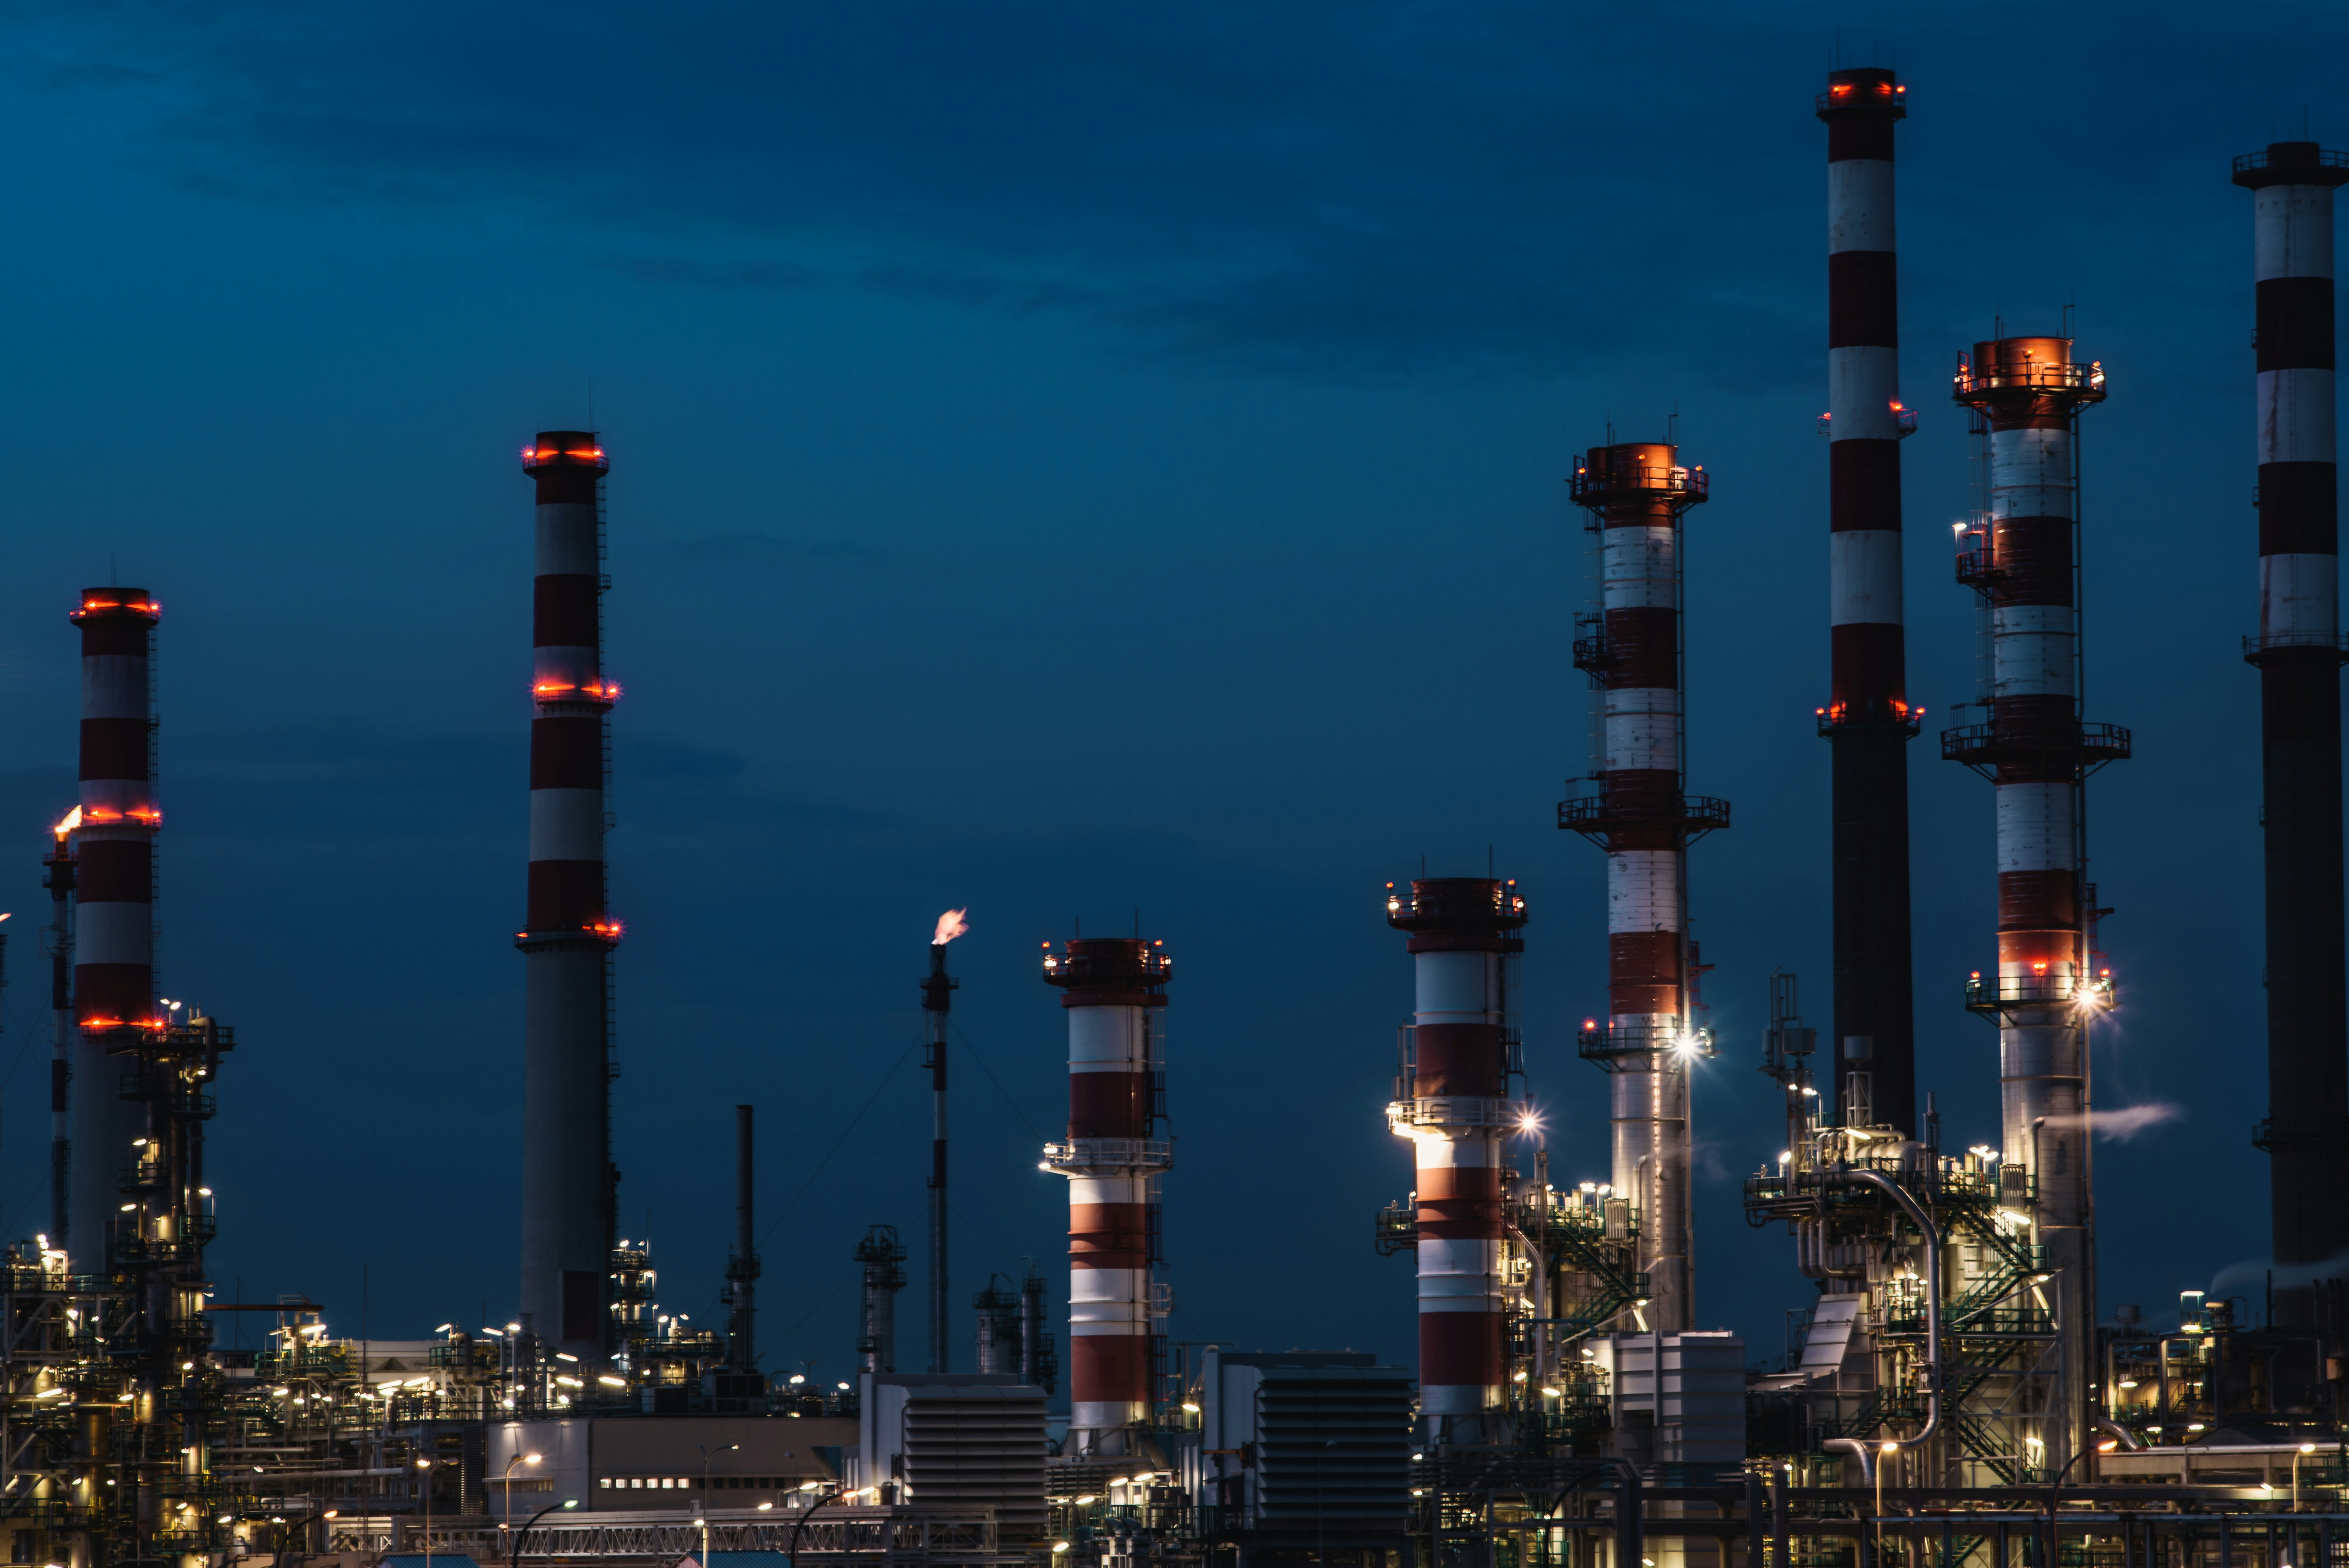
\includegraphics[width=\linewidth]{imagen1.png} 
    \end{column}
    
 
    \begin{column}{0.33\textwidth}
      \textbf{\small Energía fotovoltaica} \\
      \footnotesize Mejora la eficacia de los paneles solares. \\
      \footnotesize Modelos evaluados: \\
      \footnotesize - Uno o dos diodos \\
      \footnotesize - Modelo PV \\
      \vspace{0.5em}
      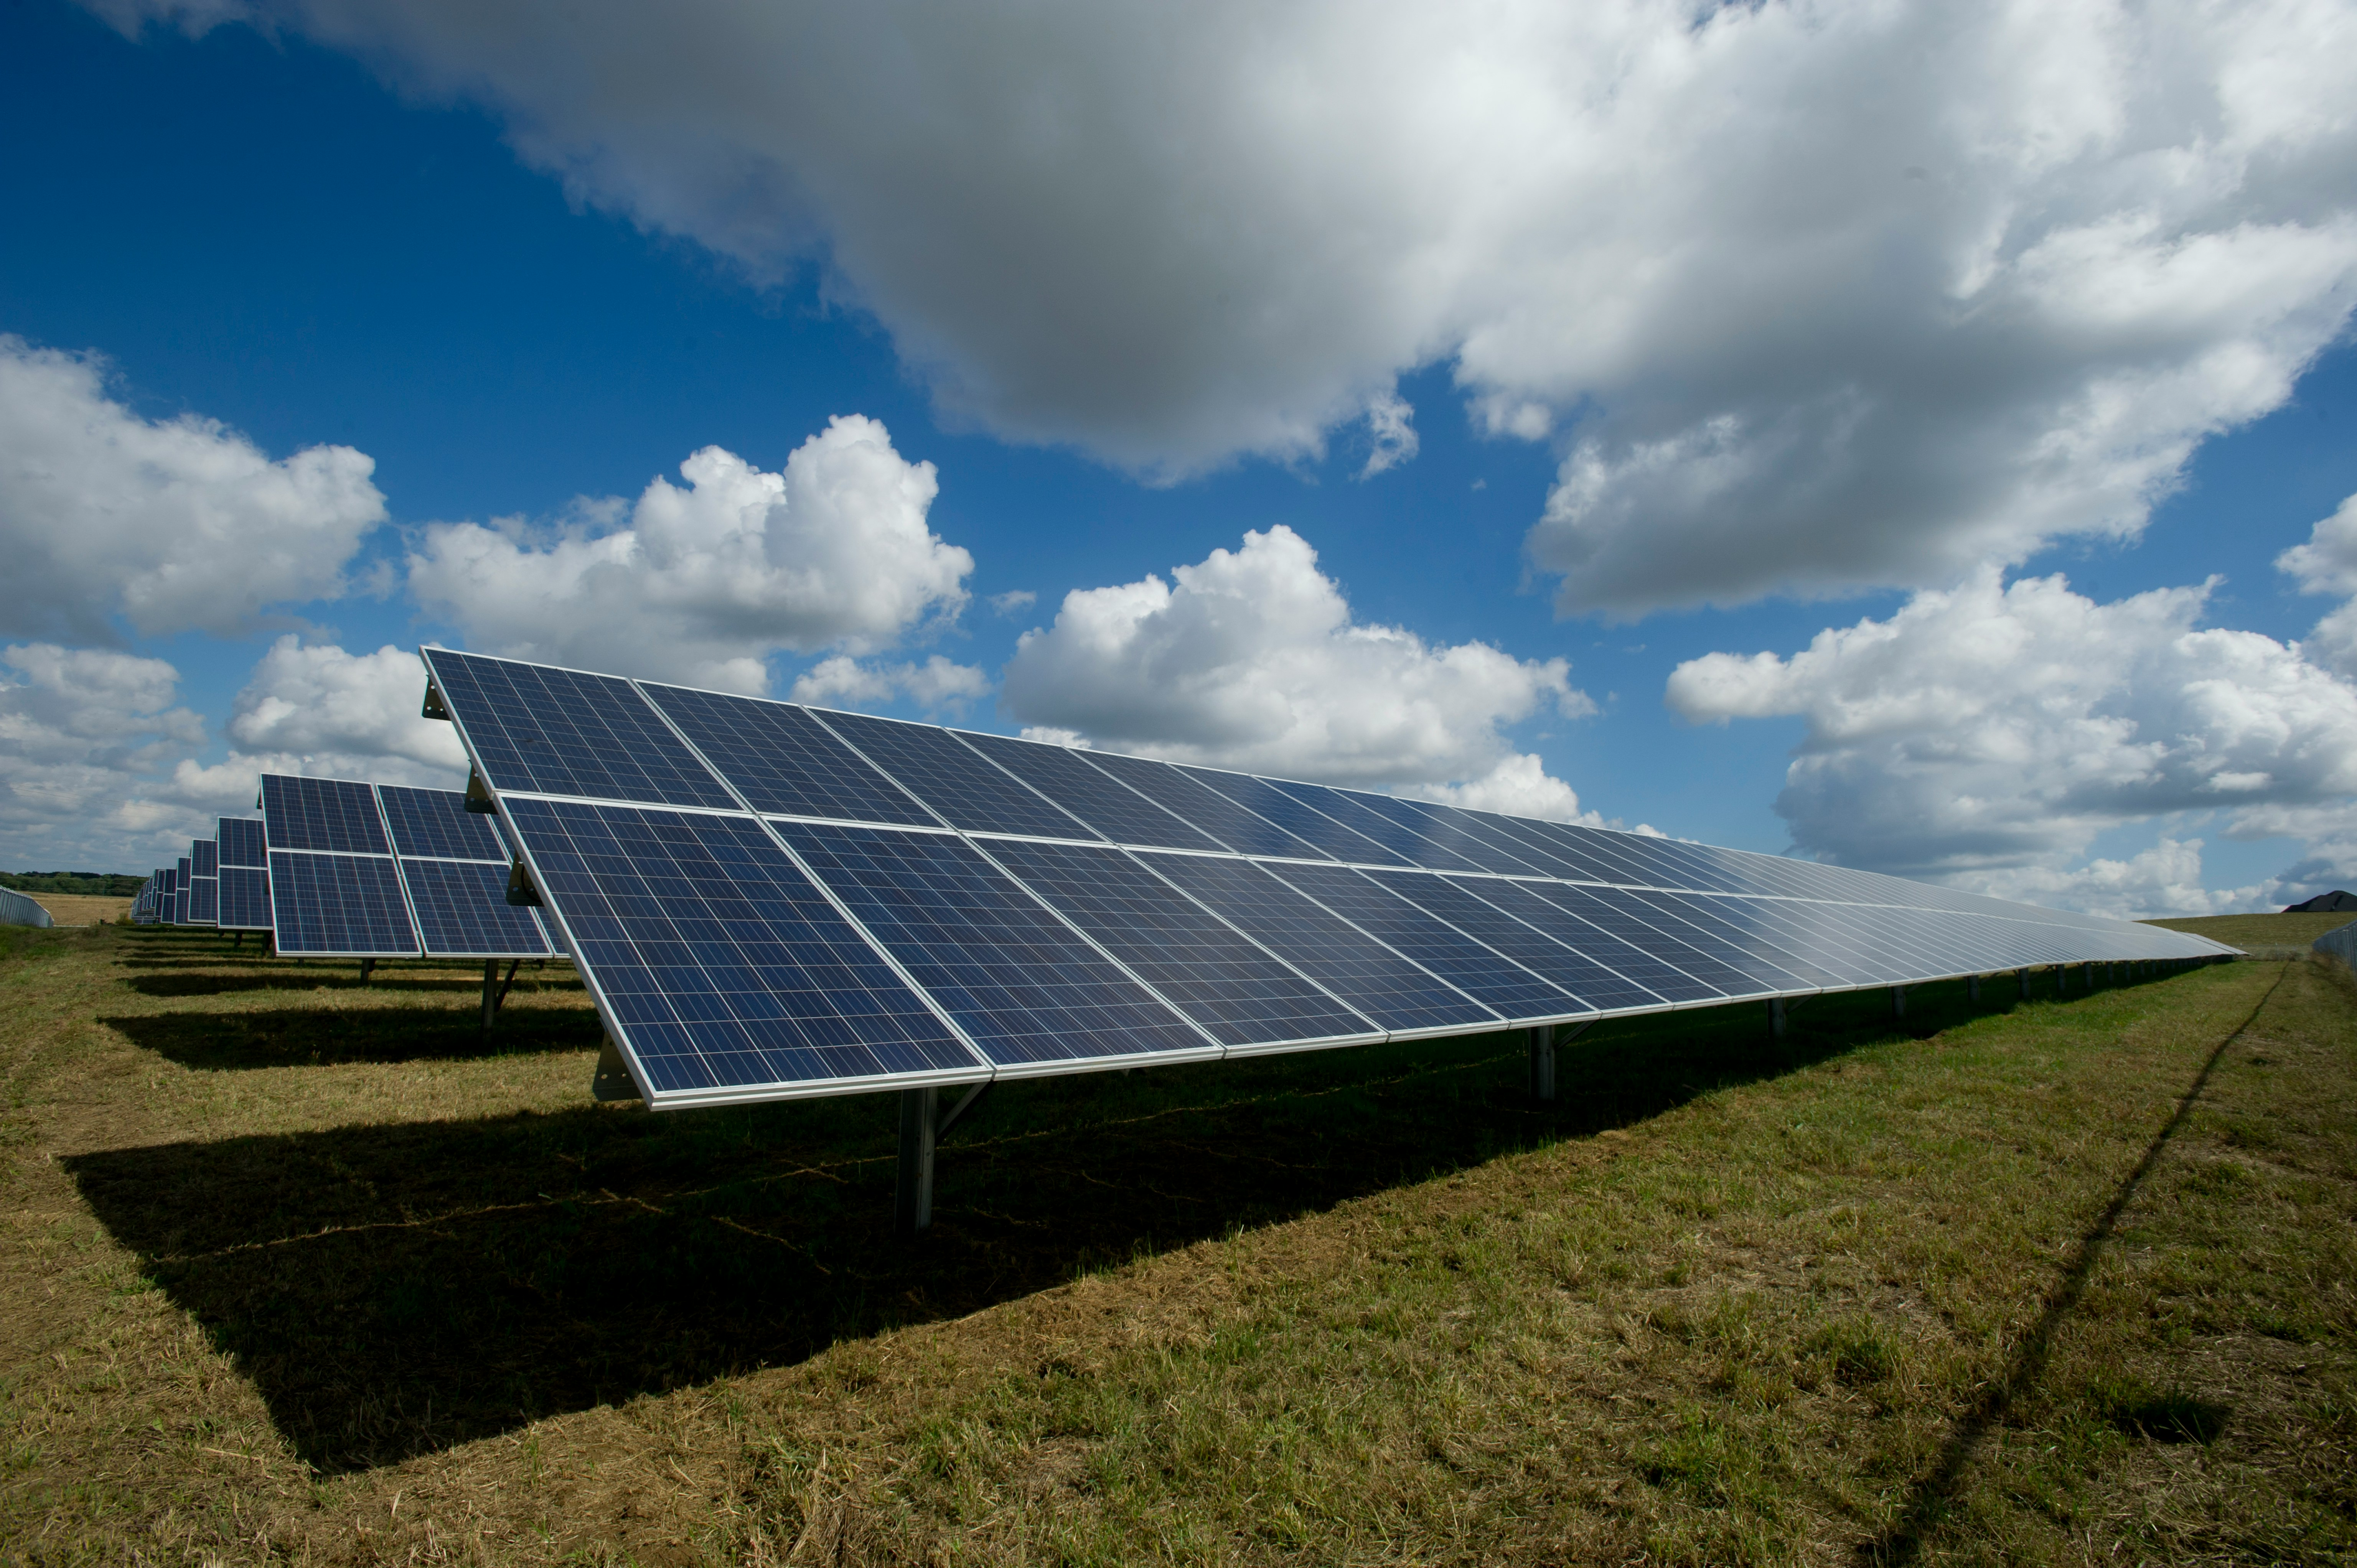
\includegraphics[width=\linewidth]{imagen2.png} 
    \end{column}
    

    \begin{column}{0.33\textwidth}
      \textbf{\small Controladores FOPID} \\
      \footnotesize Para ajustar automáticamente los parámetros en controladores avanzados.\\
      \footnotesize - Robótica \\
      \footnotesize - Aeroespacial \\
      \footnotesize - A. Industrial \\
      \vspace{0.5em}
      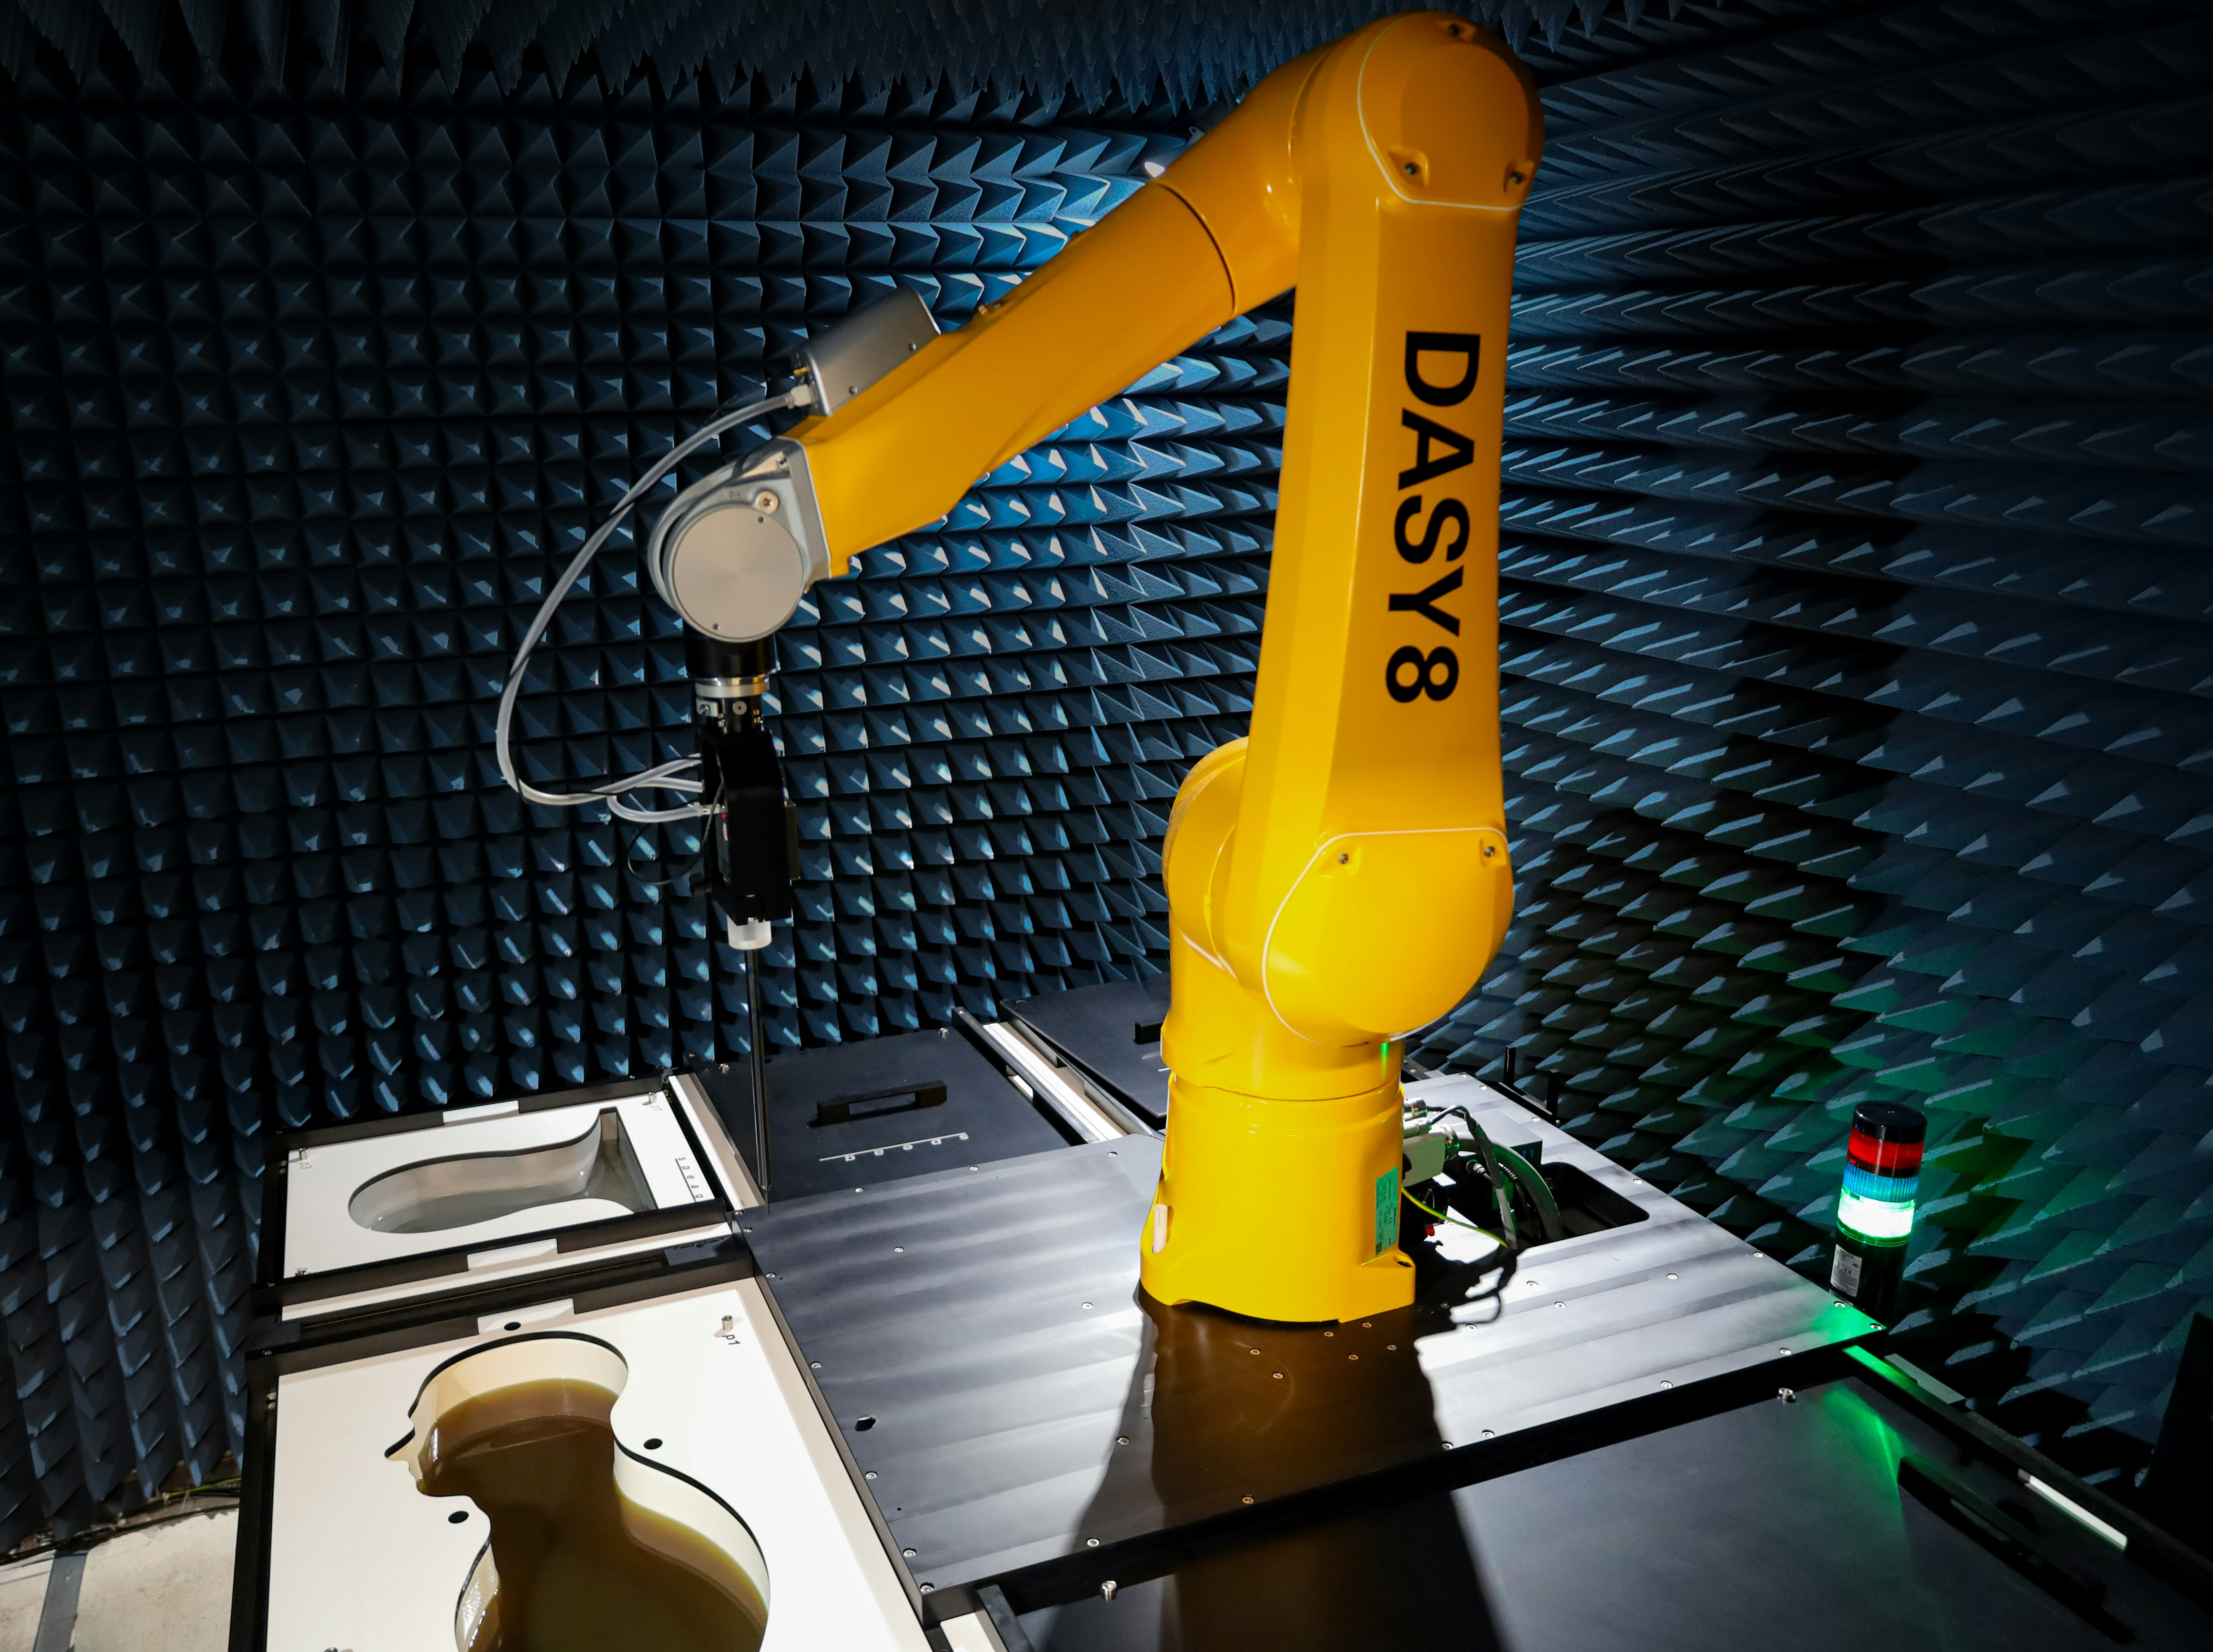
\includegraphics[width=\linewidth]{imagen3.png} 
    \end{column}
  \end{columns}
\end{frame}


\section{Conclusiones}
\begin{frame}{Conclusión}
  \begin{block}
      \justifying
      \begin{itemize}
    \justifying
          \item ALA emula los comportamientos naturales de los lemmings: migración, excavación de madrigueras, forrajeo de alimentos y evasión de depredadores.
          \item El algoritmo inicia explorando amplias soluciones y, a medida que avanza, se enfoca en mejorar las mejores encontradas, gracias a un ajuste dinámico de energía.
          \item Vuelo de Lévy y movimiento browniano permiten una búsqueda más eficiente y evitan óptimos locales.
          \item El ALA equilibra de forma eficiente la exploración y explotación, lo que lo hace altamente efectivo en problemas de optimización complejos, ajustando su estrategia a lo largo de las iteraciones.
          
      \end{itemize}
      
  \end{block}
\end{frame}


\end{document}
